\begin{solution}
\begin{enumerate}
\item {[10 points]} The requested plot is below.
\begin{center}
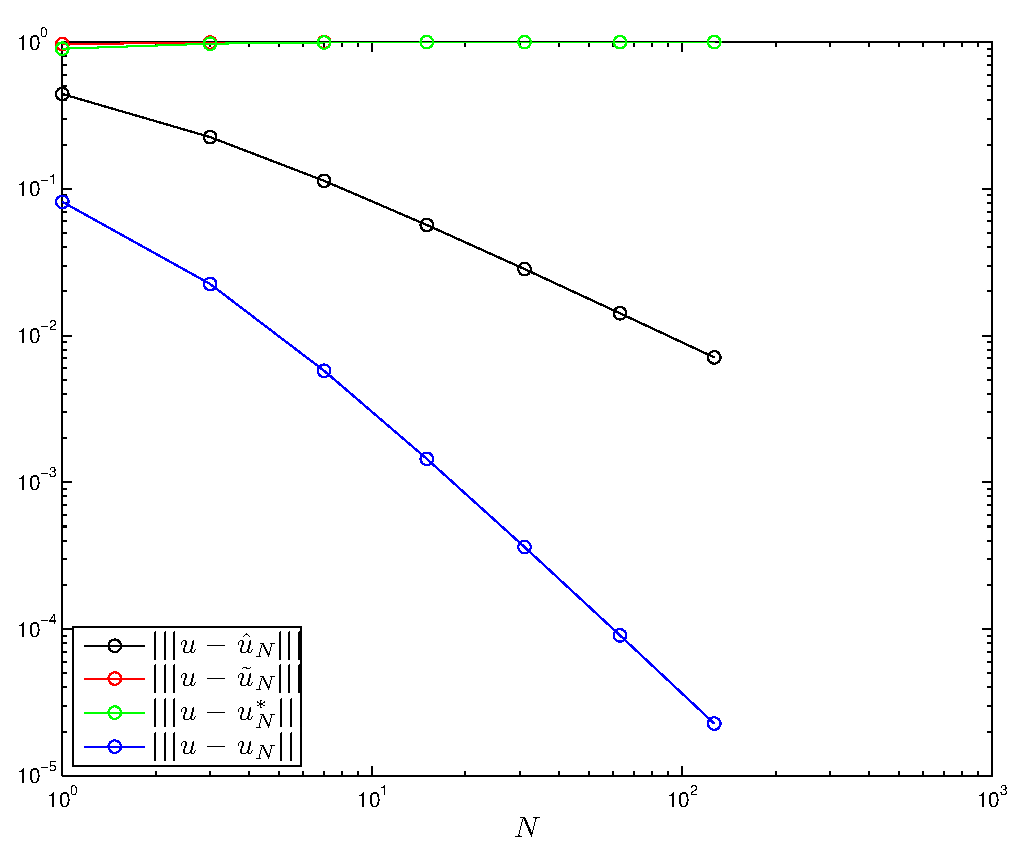
\includegraphics[scale=0.75]{hw34a.eps}
\end{center}
The code used to produce the results shown in this part and in parts (b), (c) and (d) is:

\lstinputlisting{HW34.m}

\vspace*{1em}
\item {[5 points]} The requested plot is below.
\begin{center}
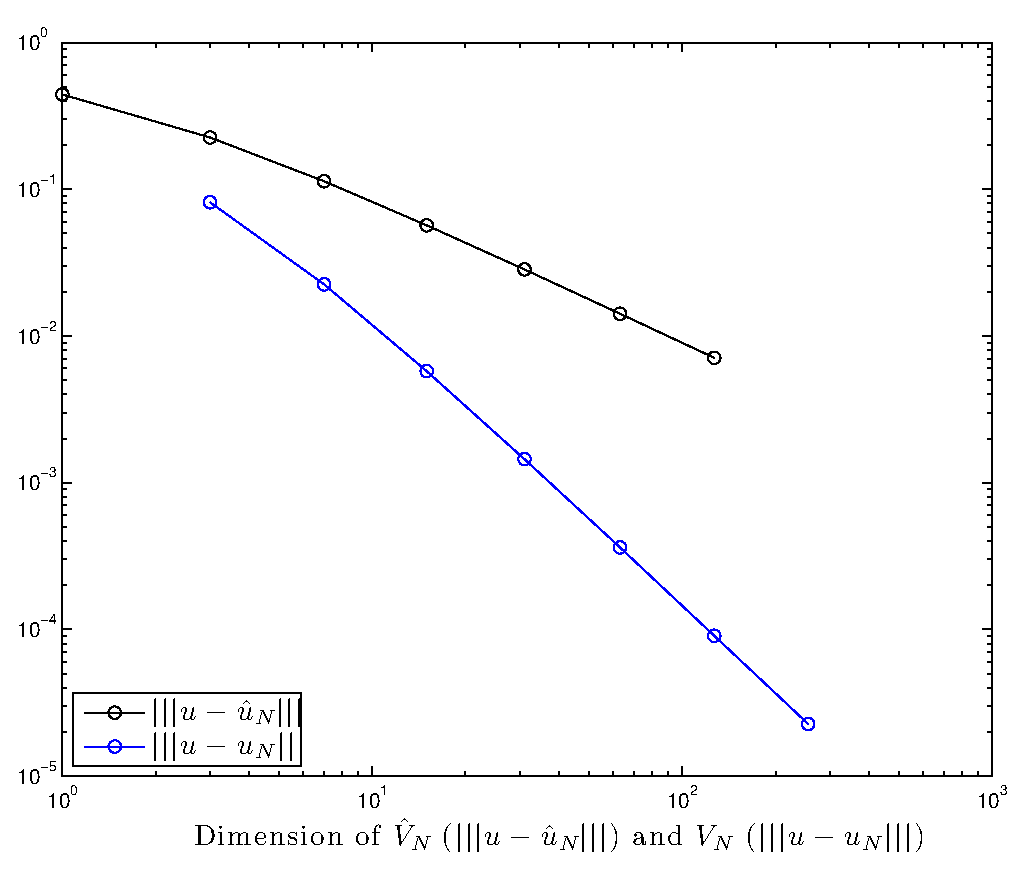
\includegraphics[scale=0.75]{hw34b.eps}
\end{center}

\vspace*{1em}
\item {[5 points]} The completed table is shown below.
\[
\begin{array}{r|r|r|r|r}
N_1 & N_2 & \rm{dim}\left(\widehat{V}_{N_1}\right) & \rm{dim}\left(\widehat{V}_{N_2}\right) & \displaystyle{{\left|\left|\left|u-\widehat{u}_{N_1}\right|\right|\right| \over \left|\left|\left|u-\widehat{u}_{N_2}\right|\right|\right|}}
\\[.75em]
\hline
1 & 3 & 1 & 3 & 1.9688
\\
3 & 7 & 3 & 7 & 1.9863
\\
7 & 15 & 7 & 15 & 1.9962
\\
15 & 31 & 15 & 31 & 1.9990
\\
31 & 63 & 31 & 63 & 1.9998
\\
63 & 127 & 63 & 127 & 1.9999
\end{array}
\]

\vspace*{1em}
\item {[5 points]} The completed table is shown below.
\[
\begin{array}{r|r|r|r|r}
N_1 & N_2 & \rm{dim}\left(V_{N_1}\right) & \rm{dim}\left(V_{N_2}\right) & \displaystyle{{\left|\left|\left|u-u_{N_1}\right|\right|\right| \over \left|\left|\left|u-u_{N_2}\right|\right|\right|}}
\\[.75em]
\hline
1 & 3 & 3 & 7 & 3.6181
\\
3 & 7 & 7 & 15 & 3.9121
\\
7 & 15 & 15 & 31 & 3.9784
\\
15 & 31 & 31 & 63 & 3.9946
\\
31 & 63 & 63 & 127 & 3.9985
\\
63 & 127 & 127 & 255 & 3.9915
\end{array}
\]
\end{enumerate}
\end{solution}

